\documentclass{article}

\usepackage{listings}
\usepackage{color}
\usepackage[utf8]{inputenc}
\usepackage{graphicx}
\usepackage[swedish]{babel}
\usepackage{fullpage}
\usepackage[T1]{fontenc}

\definecolor{mygreen}{rgb}{0,0.6,0}
\definecolor{mygray}{rgb}{0.5,0.5,0.5}
\definecolor{mymauve}{rgb}{0.58,0,0.82}

\lstset{ %
  backgroundcolor=\color{white},   % choose the background color; you must add \usepackage{color} or \usepackage{xcolor}
  basicstyle=\ttfamily\footnotesize,
  breakatwhitespace=false,         % sets if automatic breaks should only happen at whitespace
  breaklines=true,                 % sets automatic line breaking
  captionpos=b,                    % sets the caption-position to bottom
  commentstyle=\color{mygreen},    % comment style
  deletekeywords={...},            % if you want to delete keywords from the given language
  escapeinside={\%*}{*)},          % if you want to add LaTeX within your code
    extendedchars=true,              % lets you use non-ASCII characters; for 8-bits encodings only, does not work with UTF-8
    frame=single,                    % adds a frame around the code
    keepspaces=true,                 % keeps spaces in text, useful for keeping indentation of code (possibly needs columns=flexible)
    keywordstyle=\color{blue},       % keyword style
    language=Octave,                 % the language of the code
    morekeywords={*,...},            % if you want to add more keywords to the set
    numbers=left,                    % where to put the line-numbers; possible values are (none, left, right)
    numbersep=5pt,                   % how far the line-numbers are from the code
    numberstyle=\tiny\color{mygray}, % the style that is used for the line-numbers
    rulecolor=\color{black},         % if not set, the frame-color may be changed on line-breaks within not-black text (e.g. comments (green here))
    showspaces=false,                % show spaces everywhere adding particular underscores; it overrides 'showstringspaces'
    showstringspaces=false,          % underline spaces within strings only
    showtabs=false,                  % show tabs within strings adding particular underscores
    stepnumber=2,                    % the step between two line-numbers. If it's 1, each line will be numbered
    stringstyle=\color{mymauve},     % string literal style
    tabsize=2,                       % sets default tabsize to 2 spaces
    % title=\lstname                 % show the filename of files included with \lstinputlisting; also try caption instead of title
  }

  \begin{document}

  \centerline{\sc \large Modellprovning för CTL}
  \vspace{.5pc}
  \centerline{Hampus Fristedt (hamfri@kth.se)}
  \centerline{Anton Lindqvist (antoli@kth.se)}
  \vspace{2pc}

  \section{Inledning}
  Vi har implementerat ett bevissystem för CTL i Prolog. Vår implementerar
  stöder det givna, begränsade, bevissystemet och klarar alla testfall. Vår
  implementation använder sig i hög utsträckning av s.k. \emph{pattern matching}
  för att identifiera och hantera alla givna regler.

  \section{Modell}
  Vi har valt att modellera en webbsida med stöd för användarhantering i den
  utsträckningen att man kan logga in och ut. Det finns två typer av användare;
  administrator och en regelrätt användare. Både användarna har befogenhet att
  logga in och ut. Till skillnad från den regelrätta användaren har administören
  tillgång till en skyddad administrationssida.
  \begin{figure}[h!]
    \centering
    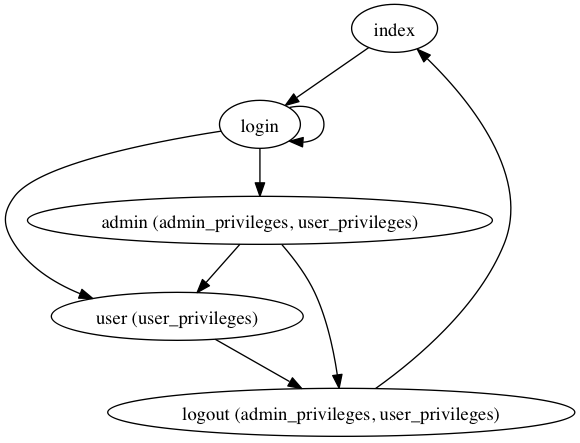
\includegraphics[scale=0.4]{model.png}
    \caption{En webbsida med användarhantering.}
  \end{figure}

  \subsection{Tillstånd}

  \begin{itemize}

    \item in: index: Startsidan synlig alla.
    \item li: login: Sida för att logga in, synlig för alla.
    \item us: user: Sida för inloggade användare.
    \item ad: admin: Sida för inloggade administratörer. 
    \item lo: logout: Sida för inloggade att logga ut. 

  \end{itemize}

  \subsection{Atomer}

  \begin{itemize}

    \item ap: admin\_privileges: Administratörsrättigheter.
    \item up: user\_privileges: Användarrättigheter.
    \item le: logged\_in: Inloggad oavsett rättigheter.

  \end{itemize}


  \newpage

  \subsection{Systemegenskaper}
  Vi har valt att konstruera två verklighetsförankrade systemegenskaper för vår
  modell. 

  \subsubsection{Giltig egenskap}
  Är du inloggad så har du antingen administratör- eller användarrättigheter.
  Detta utrycks enklast med en implikation, men vårt bevissystem för CTL saknar
  stöd för implikationer, därav har vi använt ekvivalensen:

  $$
  P \Rightarrow Q \equiv \neg P \lor Q
  $$

  \begin{figure}[h!]
    \lstinputlisting[language=Prolog]{../our_valid.txt}
  \end{figure}


  \subsubsection{Ogiltig egenskap}
  Har du loggat ut kan du inte logga in igen. Detta är givetvis falskt.

  \begin{figure}[h!]
    \lstinputlisting[language=Prolog]{../our_invalid.txt}
  \end{figure}

  \newpage

  \section{Predikat}

  \begin{itemize}

    \item \textbf{check(Transitions, Labels, State, [], and(F1, F2))}: Sant då
      femte parametern är en and-sats och både F1 och F2 är sanna.

    \item \textbf{check(Transitions, Labels, State, [], or(F, \_))}: Sant då
      den första formeln i or-satsen är sann i det givna tillståndet.

    \item \textbf{check(Transitions, Labels, State, [], or(\_, F))}: Sant då den
      andra formeln i or-satsen är sann i det givna tillståndet.

    \item \textbf{check(Transitions, Labels, State, U, ax(F))}: Sant då formeln
      F är sann i samtliga nästkommande tillstånd från tillståndet State.

    \item \textbf{check(Transitions, Labels, State, U, ex(F))}: Sant då formeln
      F är sann i något nästkommande tillstånd från tillståndet State.

    \item \textbf{check(Transitions, Labels, State, U, ag(F)}: Sant då formeln F
      är sann i samtliga tillstånd längs alla vägar tillgängliga från tillståndet
      State. 

    \item \textbf{check(Transitions, Labels, State, U, eg(F))}: Sant då formeln
      F är sann för samtliga tillstånd längs en väg tillgänglig från tillståndet
      State.

    \item \textbf{check(Transitions, Labels, State, U, ef(F))}: Sant då formeln
      F är sann i något tillstånd tillgängligt från tillståndet State.

    \item \textbf{check(Transitions, Labels, State, U, af(F))}: Sant då formeln
      F är sann i samtliga framtida tillstånd tillgängliga från tillståndet
      State.

    \item \textbf{check(\_, Labels, State, [], neg(F))}: Sant då formeln F inte
      håller.

    \item \textbf{check(\_, Labels, State, [], F)}: Sant då formeln F är en atom
      i tillståndet State.

    \item \textbf{checkAllNext(T, L, [State|States], U, F)}: Hjälpmetod för att
      verifiera att F håller i nästkommande tillstånd från tillståndet State.
      Kan användas rekursivt för att verifiera samtliga states.

    \item \textbf{getList([[State, Paths]|\_], State, Paths)}: Hjälpmetod för
      att hämta en lista ur en lista. Se exempel i programkoden.
  \end{itemize}

  \section{Programkod}
  \lstinputlisting[language=Prolog]{../src/lab2.pl}

\end{document}
